\documentclass[12pt,a4paper,openright,twoside]{book}
\usepackage[italian]{babel}
\usepackage[utf8]{inputenc}
\usepackage{fancyhdr}
\usepackage{indentfirst}
\usepackage{graphicx}
\usepackage{verbatim}

\pagestyle{fancy}


\oddsidemargin=30pt
\evensidemargin=20pt


% Sillabazione
\hyphenation{}

% Intestazione e piè di pagina
\pagestyle{fancy}\addtolength{\headwidth}{20pt}
\renewcommand{\chaptermark}[1]{\markboth{\thechapter.\ #1}{}}
\renewcommand{\sectionmark}[1]{\markright{\thesection \ #1}{}}
\rhead[\fancyplain{}{\bfseries\leftmark}]{\fancyplain{}{\bfseries\thepage}}
\cfoot{}

% Interlinea
\linespread{1.6}

\begin{document}

%
% Dedica
%
\begin{titlepage}
  % No numero di pagina
  \thispagestyle{empty}
  \topmargin=6.5cm
  \raggedleft
  \large
  %\em A Chiara
  \newpage
  % Non numera l'ultima pagina a sinistra.
  \clearpage{\pagestyle{empty}\cleardoublepage}
\end{titlepage}


\pagenumbering{roman}

\chapter*{Introduzione}
\rhead[\fancyplain{}{\bfseries
INTRODUZIONE}]{\fancyplain{}{\bfseries\thepage}}
\lhead[\fancyplain{}{\bfseries\thepage}]{\fancyplain{}{\bfseries
INTRODUZIONE}}
\addcontentsline{toc}{chapter}{Introduzione}

TODO

% Non numera l'ultima pagina a sinistra.
\clearpage{\pagestyle{empty}\cleardoublepage}

% Indice
\tableofcontents
\rhead[\fancyplain{}{\bfseries\leftmark}]{\fancyplain{}{\bfseries\thepage}}
\lhead[\fancyplain{}{\bfseries\thepage}]{\fancyplain{}{\bfseries
INDICE}}
% Non numera l'ultima pagina a sinistra.
\clearpage{\pagestyle{empty}\cleardoublepage}

\chapter{Definizione del problema}
\pagenumbering{arabic} Def problema: in un ambiente con numerose reti
senza fili eterogenee per tecnologia, politica di accesso e proprietà,
si vuole dare a un dispositivo di rete mobile la possibilità di
attraversare i campi d'azione delle suddette reti utilizzando quella
che in ogni momento risulti offrire l'accesso migliore ai
servizi. Tale dispositivo mobile viene chiamato Mobile Node (MN) e si
suppone sia dotato di più d'una interfaccia di rete senza fili. Dette
interfacce di rete (NIC) si potranno associare ognuna a una rete
differente e dovranno essere monitorate con continuità per determinare
in ogni momento quale di queste sia la più adatta ad effettuare
l'invio dei dati. La scelta di questa interfaccia designata si potrà
basare su numerosi criteri tra cui qualità del segnale radio,
percentuale di pacchetti persi, larghezza di banda offerta dal canale,
latenza di comunicazione, esigenze di sicurezza, eventuale costi
economici legati all'accesso alla rete e possibili preferenze
specificate direttamente dall'utente. L'insieme dei criteri di scelta
definisce le politiche di qualità del servizio (QoS) in uso, ovvero
l'insieme di regole e vincoli che devono essere rispettati per
garantire all'utente del MN un'esperienza soddisfacente di utilizzo
dei servizi. Le soluzioni dovranno fornire sia i meccanismi per
permettere all'utente, o alle applicazioni da lui utilizzate, di
specificare quali siano dette politiche, sia meccanismi che le
implementino.

TODO: immagine che mostri un MN che attraversa più reti e che mostra i
punti di handover.

\section{Punti critici}
\label{sec:punti-critici}
Le sezioni successive presentano gli aspetti critici del problema. La bontà di una soluzione deve essere valutata sulla base di come risolve le problematiche seguenti.

\subsection{Adattabilità}
Ogni applicazione in uso sul MN può avere le proprie esigenze di QoS,
che possono variare dalla necessità di utilizzare consistenti
quantitativi di banda alla necessità di avere una buona interattività,
misurata in termini di latenza di trasmissione dei dati. Un esempio
della prima classe di applicazioni possono essere i servizi di
Video-on-Demand (VoD), che offrono contenuti multimediali in
streaming, mentre un esempio della seconda classe è rappresentato dai
servizi Voice-over-IP (VoIP), che offrono la possibilità agli utenti
di comunicare tra di loro con chiamate audio/video sia individuali che
di gruppo. Ulteriori requisiti possono imporre un limite superiore
alla percentuale di pacchetti persi, per evitare che la qualità del
servizio non degradi oltre il limite dell'accettabile.

Le soluzioni dovranno quindi adattarsi alle necessità delle varie
applicazioni, cercando di rispettare le diverse politiche richieste da
ognuna.

\subsection{Monitoraggio}
Il concetto di qualità di servizio deve essere concretizzato in
un'insieme di limiti riguardanti metriche di comunicazione. Ad esempio
un'applicazione potrebbe richiedere che la comunicazione subisca una
perdita di pacchetti non superiore al 3\%; in questo caso
l'applicazione misura la qualità del servizio in termini di
percentuale di pacchetti persi, e impone su questa metrica un vincolo
del 3\%. Le soluzioni dovranno essere in grado di monitorare le
comunicazioni sulle varie interfacce dei MN per controllare che i
vincoli sulle metriche non vengano violati; questo richiede la
capacità di collezionare dati riguardanti queste varie metriche e la
capacità di prendere decisioni in base alle misurazioni effettuate e
alle politiche ricevute dall'applicazione. Nell'esempio precedente,
una soluzione che rilevi una percentuale di pacchetti persi superiore
al 3\% potrebbe decidere di utilizzare contemporaneamente due
interfacce di rete per limitare gli errori di trasmissione, posto che
le politiche specificate lo permettano.

\subsection{Handover}
\label{sec:handover}
Con \emph{handover} si intende il passaggio di associazione del Mobile
Node da una rete a un'altra. Lo scenario in cui le soluzioni si
troveranno ad operare sarà caratterizzato da un grado di libertà dei
MN molto ampio. Un possibile scenario è illustrato in \cite{bib:abc}:
un utente di MN comincia la comunicazione sulla rete domestica; dopo
un certo tempo esce di casa a comunicazione in corso, portando il MN
con sè. Durante il tragitto da casa alla fermata della metropolitana
il MN si disconnette dalla rete domestica e si associa alla rete
comunale, effettuando un primo handover. Quando pochi minuti più tardi
l'utente entra in metropolitana, il MN effettua un ulteriore handover
passando dalla rete comunale a quella della società dei trasporti
pubblici. Le soluzioni dovranno gestire handover di questo tipo in
maniera trasparente all'utente, ovvero senza che sia necessaria una
riconfigurazione manuale dell'applicazione o del dispositivo mobile, e
senza che venga intaccata la qualità del servizio.

L'handover è per sua natura un'operazione distruttiva che interrompe
le comunicazioni esistenti e richiede un tempo di completamento che
può arrivare all'ordine dei secondi. Tipicamente i passi che una NIC
deve completare per effettuare un handover sono:
\begin{enumerate}
\item scansione del canale per rilevare un nuovo access point,
\item associazione con il nuovo access point,
\item acquisizione di un nuovo indirizzo IP,
\item comunicazione del nuovo indirizzo IP ai vari corrispondenti, in
  modo che le comunicazioni possano continuare.
\end{enumerate}
I punti uno e due sono operazioni che appartengono al secondo livello
dello stack ISO/OSI, ovvero il livello \emph{data link}, e sono state
misurate sperimentalmente nell'ordine dei 50--400 ms
\cite{bib:misura-handoff-l2}. I punti tre e quattro sono operazioni
che appartengono al terzo livello dello stack ISO/OS, ovvero il
livello \emph{network}, e possono richiedere indicativamente almeno
300 ms \cite{bib:misura-handoff-dhcp}, perché l'assegnamento
dell'indirizzo IP da parte di un server DHCP e la comunicazione del
nuovo indirizzo a tutti gli host in contatto con il MN sono operazioni
legate alla latenza della rete.

Le soluzioni dovranno implementare meccanismi sia per ridurre questi
tempi in cui la connessione è inutilizzabile, sia per comunicare la
nuova identità del MN agli altri nodi. È importante notare che gli
altri nodi possono essere connessi a reti diverse da quella del MN e
quindi non sono applicabili meccanismi come broadcasting e
multicasting.

\subsection{Sicurezza}
In molti scenari domestici e aziendali la sicurezza della
comunicazione è spesso affidata alla sicurezza del medium in uso, ad
esempio il cavo ethernet o la crittografia della rete WiFi, e il
riconoscimento dell'identità dell'host è basata sull'indirizzo IP
dell'interfaccia di rete attiva. Queste assunzioni non sono più valide
nello scenario del problema in esame, dove numerosi MN con interfacce
di rete multiple eseguono numerosi handover attraverso reti senza
fili. Poiché queste reti verranno utilizzate da un grande numero di
individui che non possono avere relazioni di mutua fiducia, la
sicurezza è un problema centrale. Le soluzioni dovranno quindi fornire
sia meccanismi per garantire la riservatezza e l'integrità dei singoli
flussi di dati per ogni MN, sia meccanismi di identificazione e
autenticazione di ogni MN che sia indipendente dall'indirizzo IP della
rete di accesso.

\subsection{Praticità}
Nello scenario del problema sono coinvolte un gran numero di
tecnologie hardware e software che devono essere modificate il meno
possibile per permettere una realizzazione effettiva delle soluzioni
proposte in tempi e costi il più possibile contenuti.

In particolare è importante che le soluzioni siano in grado di
funzionare sui dispositivi hardware di rete esistenti, come interfacce
di rete, access point e router. Inoltre è vitale che la soluzione si
adatti ai più diversi scenari di topologia di rete, soprattutto in
quelle situazioni in cui esistono firewall e NAT che possono limitare
il traffico e la raggiungibilità degli host. Infine le applicazioni
software esistenti, dovrebbero essere in grado di funzionare senza
modifiche.

Per aiutare il passaggio graduale dell'utenza dalle soluzioni
tradizionali alle soluzioni proposte, è auspicabile che queste ultime
siano in grado di convivere con le prime utilizzando meccanismi di
fallback che garantiscano l'interoperabilità.

% Non numera l'ultima pagina a sinistra.
\clearpage{\pagestyle{empty}\cleardoublepage}

\chapter{Panoramica delle soluzioni}
\lhead[\fancyplain{}{\bfseries\thepage}]{\fancyplain{}{\bfseries\rightmark}}
L'obiettivo è di permettere a un MN di muoversi attraverso reti
wireless di natura eterogenea in maniera trasparente, ovvero senza
interrompere eventuali connessioni attive durante la transizione da
una rete all'altra. Perché questo sia possibile è necessario che ogni
MN sia a) univocamente identificato e b) universalmente raggiungibile
dagli altri nodi, in qualunque rete si trovi. Inoltre ogni MN dovrebbe
c) monitorare la qualità di ogni connessione wireless per poter
individuare la rete che offre le migliori garanzie di servizio e d)
eseguire un cambio di associazione trasparente per assicurare una
transizione senza interruzioni da una rete all'altra.

Questo capitolo presenterà le soluzioni più importanti presenti in
letteratura, senza entrare nel merito dei singoli dettagli tecnici, ma
raggruppando e catalogando per tipo i vari approcci e mostrando come
ogni soluzione affronti ognuno dei quattro punti chiave.

Le architetture si possono suddividere in due gruppi: soluzioni
\emph{single layer} e soluzioni \emph{cross layer}. Le soluzioni

\section{Soluzioni \emph{single layer}}
Le architetture seguenti sono dette \emph{single layer} perché hanno
una collocazione ben precisa nello stack ISO/OSI e operano soltanto al
loro livello di appartenenza. L'analisi di queste soluzioni mostrerà i
limiti dell'approccio single layer, limiti che saranno superati dagli
approcci \emph{cross layer} descritti nella sezione successiva.

Queste architetture coprono i principali strati dello stack ISO/OSI:
Mobile IPv6 \cite{bib:mipv6} e la sua estensione Multiple Care-of
Addresses Registration \cite{bib:mcoa} agiscono a livello
\emph{network}, Host Identity Protocol \cite{bib:hip} definisce un
livello aggiuntivo tra \emph{network} e \emph{transport}, Datagram
Congestion Control Protocol \cite{bib:dccp} e Mobile Stream Control
Transport Protocol \cite{bib:m-sctp} lavorano a livello
\emph{transport}, infine Terminal Mobility Support Protocol
\cite{bib:tmsp} e MMUSE \cite{bib:mmuse} agiscono a livello
\emph{session}.

\subsection{Mobile IPv6 e Multiple Care-of Addresses Registration}
* Home Agent nella rete fa da LR\\
* Host parlano IPv6\\
* quindi infrastrutture di rete attuali non sono adatte\\
* no multi homing, perche' il protocollo non lo permette\\
* handover tribolato\\
MCoA\\
* estensione di MIPv6\\
* permette a MN di registrare più IP address con il suo Home Agent\\
* FlowMob permette di separare flussi di traffico tra le varie NIC\\
* stessi problemi di MIPv6: tutte le infrastrutture da cambiare.

\subsection{Host Identity Protocol}
* server tipo DNS opera fuori dalla rete di accesso\\
* mappa identificatori a posizioni\\
* il layer aggiuntivo deve essere installato sia nel MN che nel
  CN.\\
* Poco pratico! Non è detto che il CN si prenda la briga di installare\\
  il layer aggiuntivo.\\

\subsection{Datagram Congestion Control Protocol}
* ogni MN annuncia il cambiamento di rete all'altro nodo\\
* funziona solo se cambiano rete uno alla volta! Due MN che cambiano
  rete simultaneamente sono irragiungibili.\\
* richiedono modifica delle applicazioni.\\

\subsection{Mobile Stream Control Transport Protocol}
Idem a DCCP.

\subsection{Terminal Mobility Support Protocol}
* SIP user agent pubblico fuori dalle reti di accesso, mappa
  user@foo.com a posizione\\
* handover lento! ogni riconfigurazione interrompe la comunicazione
  finchè MN non ha finito di comunicare con l'user agent pubblico.

\subsection{MMUSE}
* server SIP, Session Border Controller (SBC) all'interno del
  sistema autonomo, che può essere composto da più reti wireless
  eterogenee.\\
* permette di attraversare i firewall e di spostarsi da una subnet
  all'altra all'interno dello stesso AS.\\
* MN non si può muovere tra reti di diversi AS.\\

\subsection{Considerazioni}
Tutte soluzioni tranne MMUSE hanno problemi con NAT e
firewall. Bisogna usare TURN e STUN. Tutte soluzioni senza
multi-homing, tranne MCoA.

\section{Soluzioni \emph{cross layer}}
Queste architetture sono dette \emph{cross layer} perché agiscono a
multipli livelli dello stack ISO/OSI, superando i limiti delle
architetture \emph{single layer} descritte in precedenza.

Il concetto di fondo di queste architetture è utilizzare le
informazioni disponibili al livello \emph{data link} per poter
prendere decisioni efficaci di qualità di servizio ai livelli più
alti, come trasporto o sessione.

Questa sezione confronterà le soluzioni ``Media Optimization Network
Architecture'' (MONA) e ``Always Best Packet Switching'' (ABPS).

Entrambe le architetture agiscono in uno scenario in cui ci sono
numerosi Mobile Node (MN), ognuno dotato di più interaccie di rete
(NIC), che operano in un ambiente dove sono disponibili più reti
wireless, eterogenee per tecnologia e dominio. Si immagina che i
movimenti degli utenti portino i vari MN ad attraversare le aree di
copertura delle reti wireless, per cui un MN connesso ad una
determinata rete A potrebbe spostarsi in un'area in cui giungono sia i
segnali della rete A che quelli di una seconda rete B, per poi
spostarsi ulteriormente nell'area di copertura della sola rete
B. Durante questi spostamenti l'utente deve essere in grado di
utilizzare applicazioni di rete real time, come Voice over IP e Video
on Demand, senza avere ripercussioni sulla qualità dell'esperienza. Il
traffico real time deve inoltre coesistere con il traffico non real
time delle applicazioni TCP/IP tradizionali, senza per questo venirne
penalizzato.

\subsection{Media Optimization Network Architecture}
%% Breve panoramica di MONA

MONA definisce uno strato aggiuntivo, posizionato tra gli strati
\emph{network} e \emph{transport} e denominato \emph{association
  layer}, che implementa l'Association Management Protocol (AMP);
detto protocollo risiete degli host e ne gestisce i singoli
collegamenti di rete, nascondendone la molteplicità allo strato
\emph{transport} superiore.

La molteplicità di collegamenti viene sfruttata per gestire il
problema dell'\emph{handover}, ovvero del passaggio dall'associazione
con una rete all'associazione con un'altra. In MONA ogni NIC tenta di
associarsi al proprio access point, e AMP decide se utilizzare una
sola NIC, quando il collegamento è soddisfacente, o se utilizzarne più
d'una contemporaneamente, quando il monitoraggio della NIC mostra
problemi di degrado delle prestazioni di rete.

MONA inoltre propone una modifica al comportamento degli access point
per supportare più efficientemente il traffico bidirezionale tipico
delle applicazioni VoIP e una aggiunta alle frame di \emph{probe} e
\emph{beacon} per permettere ai MN di selezionare l'access point con
migliore \emph{throughput}.


\subsection{Always Best Packet Switching}
%% Breve panoramica di ABPS

TODO

Fixed server, rappresenta MN. Uso simultaneo di tutte le
NIC. Scorciatoie SIP per evitare dialoghi lenti con server
SIP. Sicurezza e identificazione: pre-shared key, flow-id e niente
REINVITE. Meccanismi a disposizione per diverse politiche: VoIP usa
error detection ed early retransmission, VoD usa più NIC
contemporaneamente per maggior banda: virtual channels per selezionare
politiche. Estensioni: ABPS-SIP e ABPS-RTP.


\subsection{Considerazioni}
Vantaggi delle due soluzioni rispetto a quelle single layer.

\clearpage{\pagestyle{empty}\cleardoublepage}


\chapter{Media Optimization Network Architecture}

Media Optimization Network Architecture (MONA) è un progetto
di... TODO

In previsione dello sviluppo delle reti ubique, MONA affronta i
problemi descritti nella sezione \ref{sec:punti-critici} con un
approccio multihoming e cross layer.

La maggior parte del sistema MONA si concentra sul QoS dei
collegamenti \emph{first hop}, ovvero i link wireless.

I requisiti di MONA per avere una buona qualità di servizio sono:
1) iniziazione dell'handover basata sul rilevamento delle
caratteristiche del link wireless, 2) eliminazione dell'interruzione
dovuta all'handover, 3) selezione dell'interfaccia ottimale.

Sfruttando più interfacce di rete, MONA affronta il problema
dell'eterogeneità dei collegamenti, permettendo flussi di dati
multipli e fornendo QoS per ognuno; le NIC multiple permettono inoltre
di gestire l'handover in modo trasparente.

L'handover viene effettuato quando il collegamento wireless in uso
viene giudicato non più soddisfacente. Per determinare la qualità di
un collegamento, MONA misura il numero di ritrasmissioni a livello
data link.

Per gestire la molteplicità di NIC e i cambi di indirizzo IP dovuti
agli handover, MONA inserisce un nuovo layer chiamato
\emph{association layer} tra il livelli rete e trasporto. Il
protocollo relativo, denominato Association Layer Protocol (AMP),
aggrega e gestisce i flussi di dati tra gli endpoint inserendo
segnalazioni di modifica di stato e informazioni di identificazione.

Considerando che le applicazioni VoIP generano un traffico simmetrico
in uplink e in downlink e che il protocollo 802.11 è stato progettato
per ottimizzare il downlink, MONA propone una modifica al protocollo
per migliorare la bidirezionalità del traffico.

Per ultimo, per evitare che alcuni access point siano sovraccarichi di
collegamenti mentre altri rimangono inutilizzati, MONA propone un
algoritmo decentralizzato per distribuire i collegamenti tra gli
access point.

Le sezioni successive analizzeranno in dettagli questi punti.

\section{Association layer}

L'Association Layer (AL) di MONA è uno strato di associazione inserito
tra i livelli rete e trasporto AL è stato implementato in questa
posizione della pila dei protocolli per motivi di compatibilità. Come
mostrato dalla figura \ref{fig:mona-association-layer}, lo strato di
associazione è superiore allo strato di rete e non interferisce con lo
stack di protocolli di dispositivi come router e access point; in
questo modo MONA può funzionare senza modifiche agli apparati di rete.

\begin{figure}[tb]
\centering
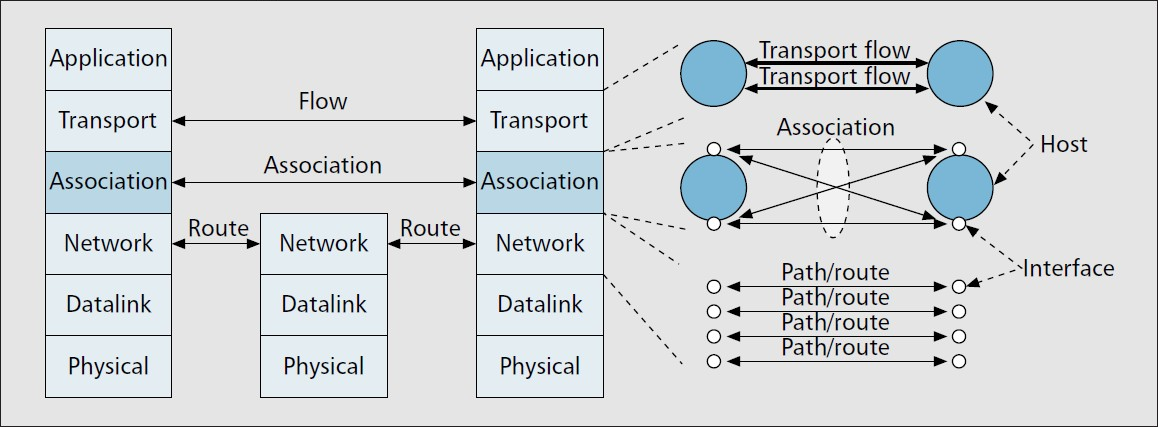
\includegraphics[width=\textwidth]{img/mona-association-layer}
\caption{\em Association layer di MONA}
\label{fig:mona-association-layer}
\end{figure}

Il protocollo Association Management Protocol (AMP) viene impiegato
dall'association layer per gestire gli stati delle associazioni tra i
vari host. Lo stato di ciascuna associazione può essere Inattivo
(Idle) quando non c'è comunicazione tra peer, Associato (Associated)
quando i due peer stabiliscono un'associazione attraverso il
three--way handshake di AMP, oppure Non Associato (No Association),
quando uno dei due peer non è in grado o rifiuta di stabilire
un'associazione. In quest'ultimo caso il layer di associazione
permette comunque la comunicazione tra gli host, assumendo un
comportamento trasparente; in altre parole, quando il tentativo di
associazione non va a buon fine, i peer comunicano attraverso lo stack
tradizionale, senza che l'estensione di associazione venga
utilizzata. Questo non permette di avere QoS tra i due peer, ma almeno
non impedisce le comunicazioni tra i dispositivi che implementano
l'Association Layer e i dispositivi tradizionali. Questa scelta
dovrebbe aiutare l'inserimento graduale dell'architettura nel mercato.

Quando due peer effettuano con successo un handshake AMP, lo strato di
associazione crea un'astrazione in cui tutti i flussi di rete tra i
due peer vengono raggruppati. Tale astrazione viene semplicemente
chiamata associazione e permette di ottimizzare le risorse di rete
condividendo le informazioni di identità dell'host tra i vari flussi
associati. L'associazione evita quindi all'host di dover ricorrere a
segnalazioni individuali per flusso ogniqualvolta venga eseguito un
handover: è infatti AL che, attraverso AMP, notifica le identità dei
flussi e delle interfacce di rete ai vari peer.

Nel caso in cui tra due peer venga stabilita un'associazione, il layer
inserisce in ogni pacchetto in uscita un header AMP posto tra l'header
e il payload IP, in modo da marcare ogni pacchetto dei flussi
dell'associazione. Tuttavia, secondo il protocollo AMP, i pacchetti di
controllo e di gestione, come le notifiche di instaurazione e di
terminazione dell'associazione, possono essere inviati
indipendentemente dai pacchetti di traffico, in modo che il layer di
associazione non debba attendere l'invio dei dati da parte degli
strati superiori per notificare il peer di eventi urgenti.

\section{QoS}
\label{sec:mona:qos}

La parte più interessante di MONA è la gestione della qualità del
servizio durante gli handover. MONA indica negli handover il punto
cruciale in cui si verifica la maggior percentuale di pacchetti persi
per un tempo abbastanza lungo da rendere impossibile la
comunicazione. Vengono considerati due tipi di packet loss: il primo
dovuto esplicitamente alla procedura di disattivazione e riattivazione
dell'interfaccia wireless durante il cambio di access point, come
descritto nella sezione \ref{sec:handover}, il secondo dovuto a
interferenze e collisioni tra pacchetti inviati da MN diversi.

Per evitare il periodo di inattività dovuto all'handover, MONA propone
di utilizzare più di un'interfaccia di rete sul MN, in modo che
durante il periodo di inattività di una, le altre siano in grado di
comunicare. Per esempio, mentre il MN sta comunicando con un peer
attraverso un'interfaccia di rete IF1, l'interfaccia di rete IF2
potrebbe cercare un'associazione di rete con un altro access point,
senza che questa attività influenzi la trasmissione dei dati
attraverso IF1. Se IF2 dovessere trovare un access point disponibile,
MN avrebbe due NIC collegate a Internet attraverso due reti
differenti; qualora il collegamento wireless di IF1 dovesse diventare
insoddisfacente, MN potrebbe dirottare il traffico in uscita da IF1 a
IF2, senza dover subire alcuna interruzione in quanto l'interfaccia
sarebbe già pronta all'uso.

MONA presenta un algoritmo per decidere quando è necessario passare
da l'invio di traffico su un'interfaccia all'invio di traffico su di
un'altra. Questo algoritmo misura la qualità del collegamento
attraverso il numero di ritrasmissioni a livello data link. Per
provare la validità di questo approccio, l'association layer di MONA e
il relativo protocollo AMP sono stati implementati nel simulatore di
rete Network Simulator 2 e sono stati condotti diversi esperimenti
virtuali per misurare l'efficacia dell'algoritmo e per determinare i
valori migliori di alcuni parametri.

Per prima cosa è necessario mostrare che il numero di ritrasmissioni a
livello data link sono una metrica per la misura della qualità di un
link più adatta dell'intensità del segnale radio.

\subsection{Ritrasmissioni L2 e intensità del segnale}

Secondo il protocollo 802.11 \cite{bib:802.11}, un nodo deve inviare
un ACK al peer ogniqualvota riceva un frame, in modo da confermare
l'avvenuta ricezione. Se il mittente non vede arrivare un ACK, ovvero
se il frame inviato o l'ACK stesso sono andati persi, allora
ritrasmette il frame. Questo meccanismo tenta la ritrasmissione del
frame fino a un numero prestabilito di volte: se il frame è più grande
di 2347 byte, viene ritrasmesso al massimo quattro volte, altrimenti
sette. Nel caso dell'architettura in questione il traffico in esame è
costituito da pacchetti VoIP, che sono di dimensione inferiore ai 400
byte; quindi ogni interfaccia ha a disposizione sette tentativi per
poter inviare il datagram VoIP all'access point. Se un link wireless è
in condizioni ottime, allora non si verificano mai errori di
trasmissione e i frame vengono inviati con successo al primo
tentativo. Quando le condizioni del link wireless cominciano a
peggiorare, possono cominciare a manifestarsi i primi packet loss, che
causeranno ritrasmissioni sporadiche. Infine, quando il link sarà in
condizioni critiche, le ritrasmissioni diverranno così frequenti da
raggiungere il limite di tentativi, provocando la perdita definitiva
del datagram.

Il primo esperimento simulato mira a trovare una relazione tra numero
di ritrasmissioni L2 e distanza del MN dall'AP. Se le due grandezze
sono correlate, allora le ritrasmissioni possono essere utilizzate al
posto della qualità del segnale. Il modello simulativo è costituito da
un MN che comunica con un CN via VoIP attraverso una rete 802.11b in
modalità infrastruttura. Entrambi i due host inviano pacchetti di 200
byte ad un intervallo di 20ms.

\begin{figure}[tb]
\centering
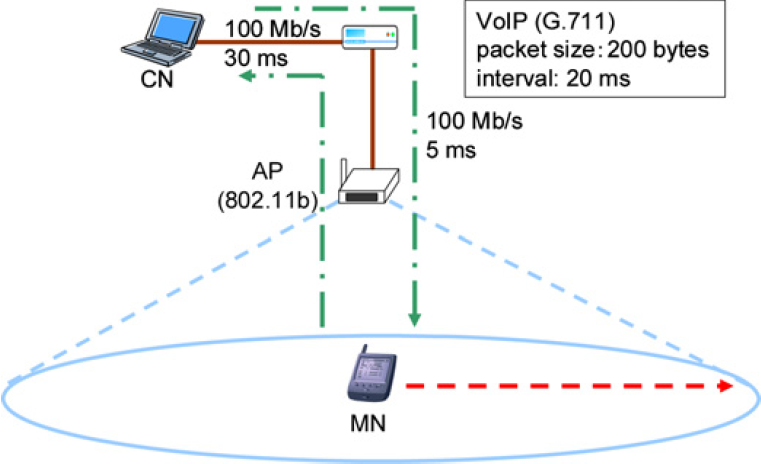
\includegraphics[width=\textwidth]{img/mona-distance-signal-strength-simulation}
\caption{\em Relazione tra distanza MN--AP e numero di ritrasmissioni e
  pacchetti persi: schema dello scenario e grafico dei risultati}
\label{fig:mona-distance-signal-strength-simulation}
\end{figure}

Il grafico della figura
\ref{fig:mona-distance-signal-strength-simulation} mostra come la
percentuale di pacchetti persi, ovvero di pacchetti scartati perché
hanno superato il numero massimo di ritrasmissioni, cresca rapidamente
a partire dalla distanza di 17 metri. Tuttavia si può notare che a
partire dai 15m le percentuali di pacchetti ritrasmessi aumentano fino
a poco sopra il 20\%. In questo scenario i 17m sono quindi la soglia
oltre la quale il segnale non è più abbastanza buono da garantire una
trasmissione senza packet loss; la simulazione mostra come il numero
di ritrasmissioni L2 permettono di rilevare questo problema prima di
incorrere nella perdita dei pacchetti. Come conclusione è lecito
affermare che il numero di ritrasmissioni L2 è una buona metrica su
cui basarsi per predirre il peggioramento del collegamento dovuto
all'indebolimento del segnale.

\subsection{Ritrasmissioni L2 e collisioni tra frame}

Poiché un secondo motivo per cui la qualità di un link wireless può
deteriorarsi è il verificarsi di collisioni tra frame spediti
simultaneamente da due o più MN, è stato condotto un esperimento per
indagare la relazione tra numero di ritrasmissioni L2 e collisioni tra
frame. Scopo della simulazione è mostrare che, eccedendo la banda
offerta da una rete wireless in modo da provocare collisioni, le
ritrasmissioni L2 aumentano di conseguenza.

Lo scenario descritto in figura \ref{fig:mona-collision-simulation} è
costituito da una rete 802.11b in cui vengono effettuate chiamate VoIP
con un numero progressivamente superiore di MN. Il traffico è
costituito da pacchetti di 200 byte inviati a intervalli di 20 ms. Dal
grafico si può notare che negli scenari in cui i MN sono presenti in
numero minore o uguale a dieci il numero di ritrasmissioni è prossimo
allo zero, mentre negli scenari in cui i MN sono undici o più il
numero di ritrasmissioni diventa via via sempre più considerevole.

\begin{figure}[tb]
\centering
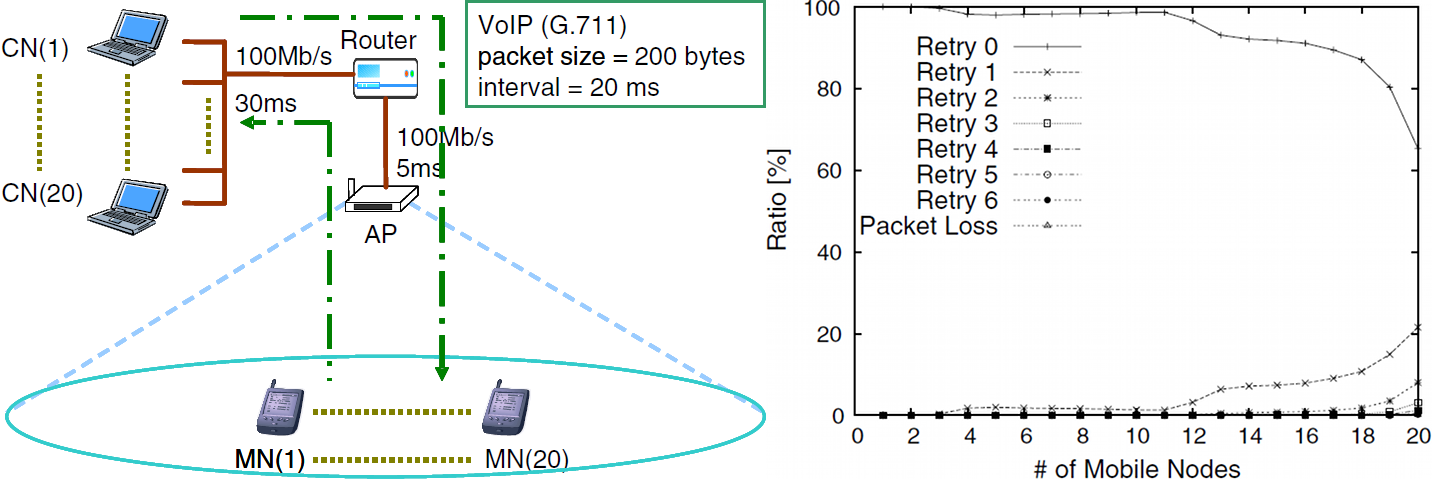
\includegraphics[width=\textwidth]{img/mona-collision-simulation}
\caption{\em Percentuale di pacchetti che vengono ritrasmessi in relazione
  al numero di MN: schema dello scenario e grafico dei risultati}
\label{fig:mona-collision-simulation}
\end{figure}

Considerando che una WLAN con banda 11MB/s può accomodare
approssimativamente 10 chiamate in cui pacchetti da 200 byte vengono
spediti a intervalli di 20ms \cite{bib:banda-wlan}, si vede che il
numero di ritrasmissioni aumenta proprio negli scenari in cui i MN
sono da undici a venti, ovvero le situazioni in cui la banda della
rete WiFI non è più in grado di reggere il carico di traffico. Questo
suggerisce che il numero di ritrasmissioni L2 è una buona metrica per
rilevare le condizioni in cui i link wireless sperimentano un alto
numero di collisioni perché la banda totale della rete wireless è
stata superata.

\section{Gestione dell'handover}

L'approccio cross--layer seguito da MONA consiste nel collezionare
informazioni sulla qualità dei link wireless a basso livello e fornire
questa informazione a uno strato superiore che decida quando e come
effettuare l'handover.

Come descritto nella sezione \ref{sec:mona:qos}, analizzare il numero
di ritrasmissioni di frame a livello data link può permettere di
predire il deterioramento di qualità di un link wireless. Questa
informazione è di basso livello, proveniendo appunto dal secondo
livello dello stack ISO/OSI. Decidere se effettuare l'handover, sulla
base di questa informazione, è invece una politica di alto livello,
che appartiene al componente aggiuntivo definito da MONA come Handover
Manager (HM). Questo componente viene implementato nello strato di
trasporto e utilizza le informazioni provenienti dal livello MAC.

\begin{figure}[tb]
  \centering
  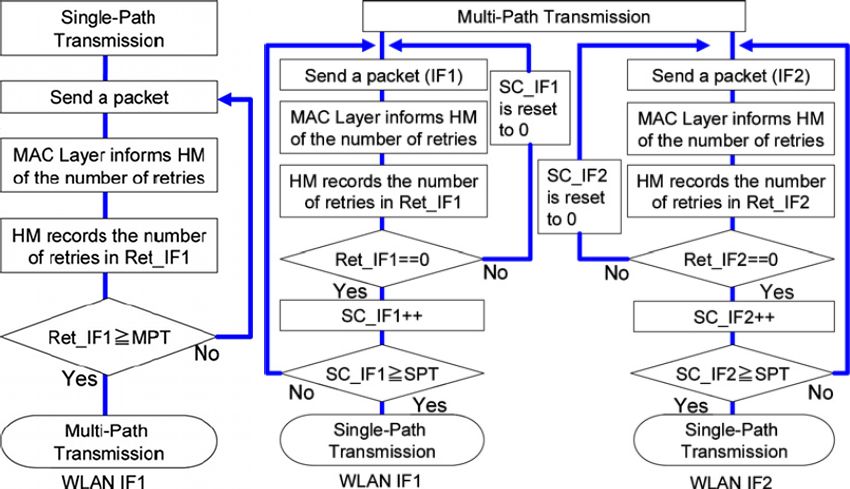
\includegraphics[width=\textwidth]{img/mona-sp-mp}
  \caption{\em Diagrammi di flusso che descrivono gli algoritmi usati da
    MONA per passare da Single Path Trasmission a Multi Path Trasmission
    (a sinistra) e viceversa (a destra).}
  \label{fig:mona:sp-mp}
\end{figure}

Nello schema proposto da MONA, quando un link viene rilevato come
problematico, l'Handover Manager utilizza le interfacce del MN
simultaneamente per prevenire il verificarsi di packet loss. Questo
utilizzo simultaneo viene chiamato Multi Path Trasmission (MPT) e
basilarmente offre sicurezza attraverso ridondanza. Quando uno dei
collegamenti in uso viene rilevato come stabile HM lo utilizza in modo
esclusivo, ritornando a quello che viene denominato Single Path
Transmission (SPT). Idealmente la modalità MPT dovrebbe essere attiva
per il tempo più breve possibile, perché l'utilizzo simultaneo di più
NIC può provocare un aumento di collisioni tra frame e determina un
aumento dei consumi di energia del dispositivo mobile.

\subsection{Da Single Path a Multi Path}

Come illustrato dal diagramma di flusso a sinistra nella figura
\ref{fig:mona:sp-mp}, si immagini un MN dotato di due interfacce
wireless IF1 e IF2. Allo stato iniziale MN comunica con il peer
attraverso l'uso esclusivo dell'interfaccia IF1; IF2 è attiva e
associata con un access point ma non riceve alcun datagram
dall'applicazione. Nel caso in cui IF2 non sia associata a nessun AP,
l'interfaccia scansiona alla ricerca di access point e si associa non
appena un AP diventa disponibile.

Durante l'uso di IF1, il MAC layer di IF1 informa HM del numero di
ritrasmissioni L2 che sono state necessarie per inviare ogni frame,
oppure comunica che il numero di ritrasmissioni massimo è stato
superato e che il frame è stato scartato. In questo modo HM viene a
conoscenza della condizione del link pacchetto per pacchetto ed è in
grado di decidere se la qualità del collegamento è diventata
insoddisfacente. Questa decisione viene presa confrontando il numero
di ritrasmissioni dell'ultimo frame, che nel diagramma è denominato
Ret\_IF1, con un valore soglia, superato il quale HM passa alla
modalità Multi Path Trasmission.

\subsection{Da Multi Path a Single Path}

Quando HM utilizza la modalità Multi Path Trasmission invia ogni
datagram ricevuto dall'applicazione a entrambe le interfacce,
raddioppiando il carico di rete e causando un incremento nelle
richieste energetiche del dispositivo mobile. Per questi motivi MPT
viene considerata una modalità d'emergenza, in cui HM deve operare per
il minor di tempo possibile.

Come in modalità SPT un alto numero di ritrasmissioni di un frame
viene considerato un indicatore del degrado di qualità del link, in
modalità MPT l'assenza di ritrasmissioni L2 viene considerato un
indice di stabilità del link. Il diagramma di destra della figura
\ref{fig:mona:sp-mp} mostra questo processo: ogni pacchetto viene
inviato simultaneamente su IF1 e IF2, che concorrentemente lo
inoltrano sul link wireless. Se il numero di ritrasmissioni di
un'interfaccia è zero, HM incrementa un valore denominato Stability
Counter (SC\_IFi), altrimenti lo reimposta a zero. Il valore SC viene
utilizzato come metrica discriminante per passare da MPT a SPT: quando
oltrepassa un certo valore soglia $s$ significa che il collegamento
wireless è stato in grado di inviare $s$ frame senza che fossero
necessarie ritrasmissioni, per cui può essere considerato stabile. La
prima interfaccia che giunge a una condizione in cui è considerata
stabile, viene selezionata da HM per essere utilizzata nuovamente in
modalità SPT.

Un problema introdotto dalla modalità MPT riguarda la ricezione di
paccheti duplicati dal peer del MN. Poiché lo stesso pacchetto viene
inviato su due interfacce connesse a reti differenti, i pacchetti
duplicati possono essere ricevuti fuori ordine, a causa delle diverse
condizioni delle due reti. La soluzione utilizzata in MONA marca ogni
pacchetto con un numero di sequenza, in modo che un nodo possa
scartare pacchetti ricevuti che possiedono un numero di sequenza
vecchio.

\section{Esperimenti simulati}

Gli ideatori di MONA ne hanno valutato l'efficacia implementando
l'Handover Manager nel Network Simulator Version 2 \cite{bib:ns-2}
(versione 2.27) e conducendo una serie di simulazioni volte a
determinare se l'approccio funziona e quali valori soglia sono più
efficaci per gli algoritmi SPT/MPT.

\begin{table}
  \centering
  \begin{tabular}[bt]{|llll|}
    \hline
    Qualità & Buona & Media & Scarsa          \\
    \hline
    Delay (ms) & $<150$ & $150-400$ & $>400$ \\
    Jitter (ms) & $<20$ & $20-50$ & $>50$    \\
    Packet loss (\%) & $<1$ & $1-3$ & $>3$   \\
    \hline
  \end{tabular}
  \caption{\em Vincoli qualitativi considerati durante la simulazione.}
  \label{tab:mona:vincoli}
\end{table}

I vincoli qualitativi che sono stati considerati durante lo
svolgimento delle simulazioni per valutare la bontà dei risultati sono
riassunti in tabella \ref{tab:mona:vincoli}; l'obiettivo è di
mantenere la latenza tra i peer sotto i 150 ms, il jitter sotto i 20
ms e la percentuale di pacchetti persi sotto il l'1\%.

\subsection{Modello simulativo}

Gli esperimenti sono stati condotti sul modello schematizzato in
figura \ref{fig:mona:qos-sim-model}

\begin{figure}[tb]
  \centering
  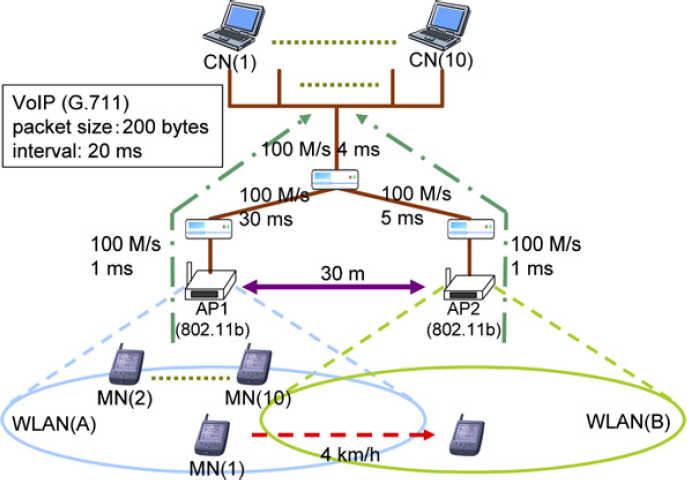
\includegraphics[width=\textwidth]{img/mona-qos-sim-model}
  \caption{\em Modello per la simulazione in NS2.}
  \label{fig:mona:qos-sim-model}
\end{figure}

Un Mobile Node (MN), equipaggiato con due interfacce di rete IF1 e
IF2, si sposta attraverso due WLAN differenti, ovvero dalla WLAN A
alla WLAN B. Durante l'handover vengono analizzati la percentuale di
pacchetti persi e il traffico di rete. Le due WLAN sono di tipo
802.11b e formano sottoreti differenti, in modo che le interfacce di
rete ricevano indirizzi IP diversi da ogni WLAN. Dieci MN sono
associati alla WLAN A e comunicano con altrettanti CN, mentre un solo
MN si sposta dalla WLAN A alla WLAN B, alla velocità di 4 Km/h, ovvero
a passo d'uomo. Tutti gli MN inviano pacchetti di 200 byte a
intervalli di 20 ms. Il delay tra peer è diverso a seconda della WLAN
a cui i MN sono associati: attraverso WLAN A è impostato a 35 ms,
mentre WLAN B 10 ms.

\subsection{Pacchetti persi}
\label{sec:mona:sim-packet-loss}

La prima analisi mira a individuare i valori migliori per le
ritrasmissioni di frame da utilizzare per le soglie di passaggio da
Single Path a Multi Path $v_{MPT}$ e da Multi Path a Single Path
$v_{SPT}$. Come da tabella \ref{tab:mona:vincoli} si sono cercati
valori in cui il packet loss misurato è minore del 3\%.

\begin{figure}
  \centering
  \begin{tabular}{cc}
    a) & 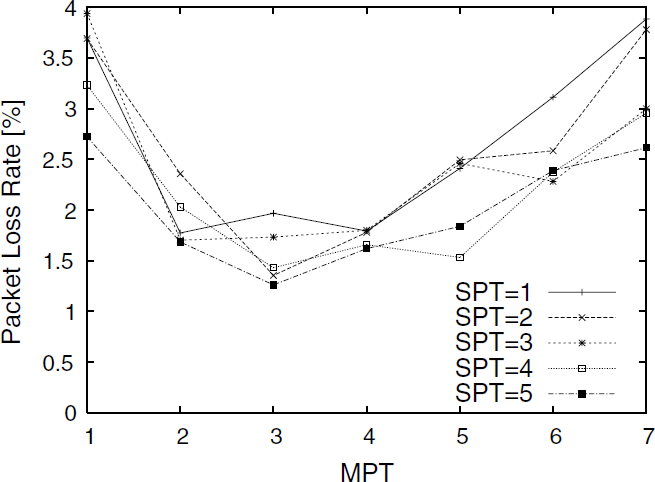
\includegraphics[width=9cm]{img/mona-sim-packet-loss-rate}  \\
    b) & 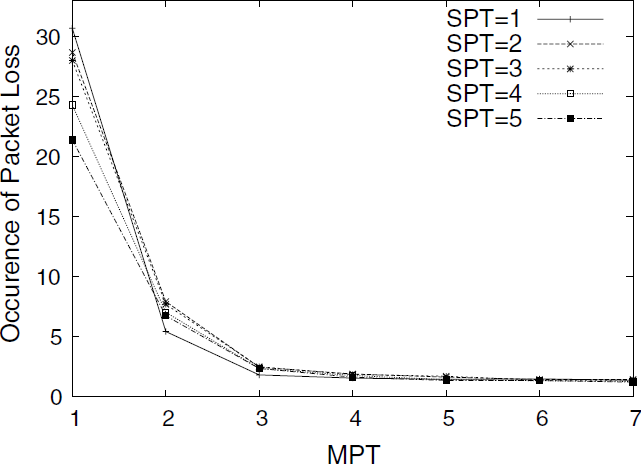
\includegraphics[width=9cm]{img/mona-sim-packet-loss-occur} \\
    c) & 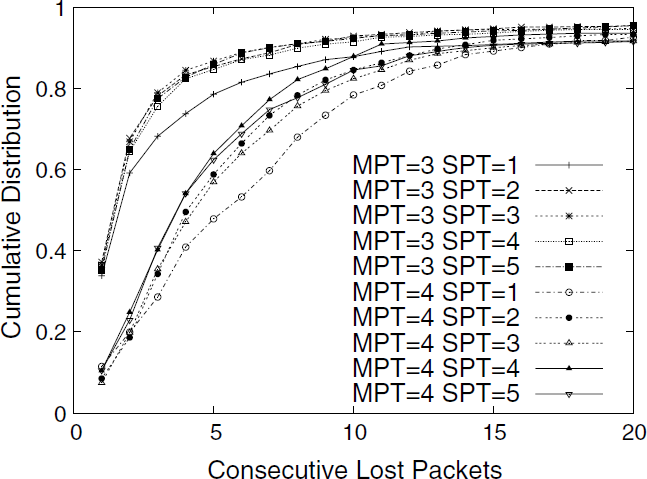
\includegraphics[width=9cm]{img/mona-sim-packet-loss-distrib}  \\
  \end{tabular}
  \caption{\em Misurazioni durante l'handover di a) percentuale di
    pacchetti persi, b) numero medio di occorrenze di pacchetti persi,
    c) distribuzione di pacchetti persi consecutivamente.}
  \label{fig:mona:qos-sim-packet-loss}
\end{figure}

Nel grafico a) della figura \ref{fig:mona:qos-sim-packet-loss} sono
mostrate le percentuali di pacchetti persi durante l'handover per
tutte le combinazioni di valori di SPT e MTP.  Le percentuali minori
del 2\% sono state misurate in corrispondenza dei valori 3 e 4 di MPT,
indifferentemente dal valore di SPT.  Che nella misura dei pacchetti
persi SPT sia un valore meno critico non stupisce, perché è il valore
che determina il ritorno alla modalità Single Path. MPT invece
determina il momento in cui HM passa alla modalità Multi Path e la
tempistica giusta è fondamentale. In particolare, si vede che quando
MPT è impostato a un valore troppo basso come 1 e 2, la percentuale di
pacchetti persi è alta come quando il valore è troppo alto (maggiore
di 4). Per approfondire il problema bisogna considerare il grafico b),
dove viene mostrato il numero di occorrenze di pacchetti persi, dove
ogni occorrenza è o un singolo pacchetto perso o una serie di
pacchetti persi. Dall'andamento del grafico si vede che con valori MPT
minori di 3 il numero di occorrenze è molto alto, ovvero ci sono
tanti pacchetti persi singolarmente, mentre per valori di MPT maggiori
di 4 il numero di occorrenze è molto basso; correlando questo dato con
quello del grafico a) dove la percentuale di pacchetti persi per
valori di MPT maggiori di 4 è molto alto, si conclude che con MPT alto
la comunicazione soffre di perdita di sequenze intere di pacchetti.

La spiegazione è da ricercarsi nella conformazione della rete: WLAN B
ha una latenza minore di WLAN A e i paccheti inviati attraverso di
essa arrivano prima dei pacchetti inviati attraverso la prima. Quando
HM è nel suo stato iniziale, invia numerosi pacchetti attraverso
l'interfaccia associata con WLAN A. L'access point relativo deve
gestire questo traffico insieme a quello degli altri dieci MN, per cui
i tempi di accodamento nel buffer del dispositivo cominceranno ad
essere rilevanti. Quando MPT ha un valore alto, HM attende che le
ritrasmissioni L2 arrivino al limite massimo e solo in quel momento
passa alla modalità Multi Path; passando a tale modalità invia un
frame attraverso WLAN B mentre nella coda di trasmissione dell'access
point sono ancora presenti numerosi frame precedenti. Poiché WLAN B ha
una latenza migliore e una congestione migliore di WLAN A, l'ultimo
frame arriverà a destinazione prima dei frame precedenti ancora
accodati; questi frame al loro arrivo verranno scartati come scaduti
perché hanno un numero di sequenza minore dell'ultimo pacchetto
ricevuto dal MN.

Nelle comunicazioni VoIP la perdita di una sequenza di pacchetti è più
grave della perdita di un pacchetto singolo. Analizzando la
distribuzione delle sequenze di pacchetti persi nel grafico c) della
figura \ref{fig:mona:qos-sim-packet-loss}, si nota che i valori più
bassi si hanno con MPT uguale a 3 e SPT uguale a 4.

\subsection{Carico di rete}

Se da una parte è necessario trovare i valori di MPT e SPT che
permettano di soddisfare al meglio i requisiti di QoS della tabella
\ref{tab:mona:vincoli}, dall'altra la modalità Multi Path è onerosa in
termini di carico di rete ed è necessario trovare un compromesso tra
qualità e utilizzo del medium.

\begin{figure}[tb]
  \centering
  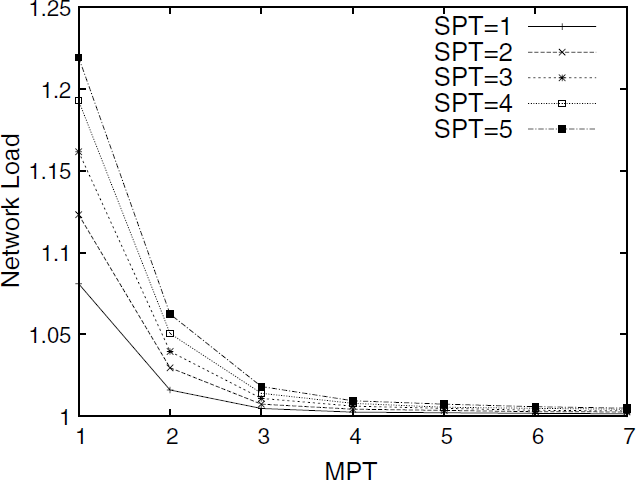
\includegraphics[width=10cm]{img/mona-sim-network-load}
  \caption{\em Analisi del traffico di rete durante l'handover}
  \label{fig:mona:sim-network-load}
\end{figure}

La figura \ref{fig:mona:sim-network-load} mostra i diversi carichi di
rete in relazione alle varie combinazione di MPT e SPT. Quando sia MPT
che SPT sono piccoli il carico di rete è relativamente basso, perché
HM passa facilmente alla modalità Multi Path, ma ritorna altrettanto
facilmente alla modalità Single Path. In contrasto, il carico di rete
massimo si ha quando MPT è basso e SPT è alto, perché HM passa
immediatamente in Multi Path e torna a Single Path con molta
difficoltà. Dalle prove condotte precedentemente (sezione
\ref{sec:mona:sim-packet-loss}) i valori più appropriati per MPT e SPT
sono risultati rispettivamente 3 e 2 e con queste costanti il carico
di rete durante il Multi Path è solo 1,004 volte il carico in Single
Path; in numeri, con un traffico di 80 kb/s in Single Path si ha un
traffico di 80,32 kb/s in Multi Path. Questo dimostra che i valori più
adatti a fornire QoS sono pienamente accettabili dal punto di vista
dell'incremento del carico di rete.

\subsection{Variazione nel ritardo dei pacchetti}

La variazione nel ritardo dei pacchetti, comunemente detta
\emph{jitter}, è un fenomeno che influenza la qualità delle
comunicazioni VoIP e dovrebbe essere al di sotto dei 50 ms, come da
tabella \ref{tab:mona:vincoli}. Nonostante MONA punti a mitigare la
perdita di pacchetti, è stato studiato l'effetto dei differenti valori
di MPT sul jitter.

\begin{table}
  \centering
  \begin{tabular}[bt]{|lllllll|}
    \hline
    Ritrasmissioni & 1 & 2 & 3 & 4 & 5 & 6                 \\
    \hline
    Jitter (ms) & 11,6 & 22,9 & 35,4 & 50,6 & 70,8 & 91    \\
    \hline
  \end{tabular}
  \caption{\em Jitter medio in relazione alle ritrasmissioni L2.}
  \label{tab:mona:jitter}
\end{table}

La tabella \ref{tab:mona:jitter} mostra i valori di jitter
relativamente al numero di ritrasmissioni di frame. Per avere valori
accettabili sotto i 50 ms è necessario che le ritrasmissioni siano al
massimo tre. Oltre questo valore i pacchetti cominciano ad accodarsi
nel buffer dell'interfaccia e subiscono variazioni nel ritardo. Il
valore migliore di MPT selezionato dalle prove precedenti è tre,
quindi l'utilizzo di MONA dovrebbe migliorare anche gli effetti sul
jitter.

\begin{figure}[tb]
  \centering
  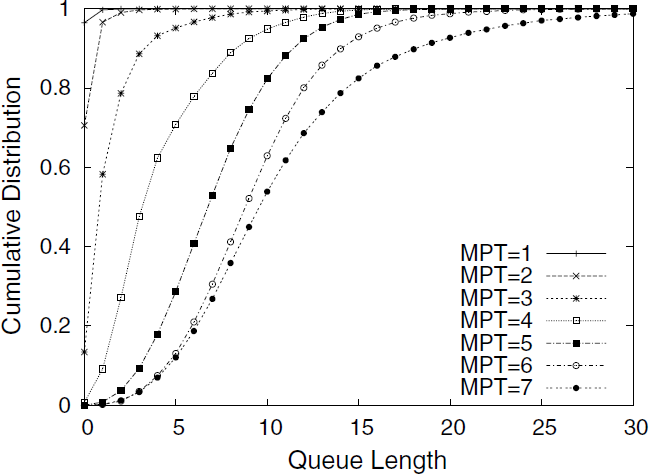
\includegraphics[width=10cm]{img/mona-sim-queue-length}
  \caption{\em Distribuzione cumulativa della lunghezza della coda di
    pacchetti nel buffer dell'interfaccia.}
  \label{fig:mona:sim-queue-length}
\end{figure}

La figura \ref{fig:mona:sim-queue-length} mostra la distribuzione di
probabilità della lunghezza della coda dei pacchetti nell'interfaccia
IF1 quando HM passa alla modalità MTP. Si può notare come a valori di
MTP crescenti la probabilità che la coda sia corta tenda a zero,
ulteriore conferma che i valori di MTP e jitter sono direttamente
correlati.

%% POSSIBILI AGGIUNTE

% Fair uplink and downlink in a WLAN.

% AP Selection: Load imbalance problem.

\section{Conclusioni}

TODO.

% DA QUI

\clearpage{\pagestyle{empty}\cleardoublepage}

\chapter{Always Best Packet Switching}
TODO: breve presentazione. Esempio: Always Best Packet Switching
(d'ora in avanti ABPS) è frutto di una ricerca in corso all'Università
di Bologna, etc. etc.

TODO: obiettivo in breve.

L'architettura offre i servizi di QoE e sicurezza illustrati nella
sezione \ref{sec:punti-critici} alle applicazioni multimediali basate
sui protocolli SIP e RTP, con l'obiettivo di permetterne l'utilizzo in
un contesto di mobilità urbana attraverso reti eterogenee per
tecnologia, amministrazione e costo, anche con topologie contemplanti la
presenza di NAT e firewall.

\section{Session Initiation Protocol}

ABPS utilizza il protocollo SIP e ne definisce un'estensione,
denominata ABPS-SIP. Per illustrare ABPS è quindi necessario trattare
il protocollo SIP nei punti salienti che riguardano l'architettura in
esame.

Questa sezione presenta quindi una panoramica del protocollo SIP,
mostrando i ruoli degli host, la gestione della sessione e alcuni
limiti dovuti alla presenza di firewall e NAT. Successivamente verrà
mostrato come ABPS estende il protocollo SIP per superare questi
limiti e i dettagli della soluzione.

\subsection{Panoramica}

Il protocollo SIP è utilizzato per creare il contesto di una
comunicazione tra due o più entità di rete. Per mezzo di SIP due host
possono venire a conoscenza l'uno dell'altro (ovvero conoscere i
rispettivi indirizzi IP) e accordarsi sui parametri della sessione di
comunicazione, dopo di che il trasferimento dati avviene in modo
diretto, secondo le modalità concordate.

\subsection{Agenti SIP}

Tra i vari ruoli che SIP prevede per gli host in gioco, la trattazione
di ABPS richiede di illustrare gli User Agent Client (UAC), gli User
Agent Server (UAS) e i Back-to-back User Agent (B2BUA).

\paragraph{User Agent Client.}
È definito come un'entità logica che crea nuove richieste SIP e le
invia attraverso la rete all'User Agent Server. Per esempio,
un'applicazione VoIP che inizi una chiamata prende il ruolo di UAC,
perché genera e spedisce la richiesta di invito.

\paragraph{User Agent Server.}
È definito come un'entità logica che crea le risposte alla richieste
ricevute. Un esempio di UAS è il server che risponde alle richieste di
registrazione degli utenti (Registrar).

\paragraph{Back-to-back User Agent.}

È definito come un'entità logica che riceve le richieste da un client
(UAC) e si comporta come se fosse un server (UAS), ma invece di
rispondere direttamente, inoltra la richiesta a un server (UAS); nel
dialogo con il client si comporta come server, mentre nel dialogo con
il server si comporta da client. In altre parole, un B2BUA è un
intermediario tra UAC e UAS: UAC crede che il B2BUA sia l'UAS,
dall'altra parte l'UAS crede che il B2BUA sia l'UAC.

\subsection{Gestione delle sessioni SIP}

In uno scenario VoIP, l'applicazione UAC utilizza il protocollo SIP
per inviare all'UAS un messaggio REGISTER, che segnala che l'utente è
collegato e pronto a ricevere e inviare chiamate. Dopo che l'UAC si è
registrato al servizio, può instaurare una sessione mediante un
messaggio INVITE, che specifica l'identificativo dell'utente da
contattare e i dati dell'utente chiamante; ricevuta la richiesta
INVITE, il server recupera l'indirizzo IP dell'utente specificato e
instaura una sessione tra i due partecipanti, che possono comunicare
direttamente mediante protocollo RTP.

Nel caso in cui il chiamante modifichi il proprio stato durante una
conversazione, l'applicazione invia un nuovo messaggio INVITE
contentente i parametri aggiornati, per permettere al server di
reinstaurare la sessione con le nuove caratteristiche.

Il meccanismo di re-INVITE è intrinsecamente lento: il mittente deve
contattare il server, il server deve a sua volta contattare il
destinatario e solo a quel punto la comunicazione tra mittente e
destinatario può continuare nella nuova sessione. Nonostante questo
procedimento possa avvenire in automatico, ovvero senza intervento
manuale dell'utente, la comunicazione vocale deve essere interrotta
finché non viene instaurata la nuova sessione, condizionando
l'esperienza utente.

ABPS definisce delle scorciatoie di segnalazione per rendere diretto il
procedimento di re-INVITE; i partecipanti possono modificare i
parametri della sessione in cui sono coinvolti senza dover
interpellare il server e quindi evitando di dover attendere che la
sessione sia reinstaurata.

\subsection{Problematiche dovute a Firewall e NAT}

Il protocollo SIP si limita a creare il contesto della comunicazione,
permettendo ai partecipanti di specificare le caratteristiche della
sessione, instaurata la quale lo scambio di dati avviene in maniera
diretta tra i due host. Alla luce di ciò, NAT e firewall sono
impedimenti perché non permettono a un host di essere direttamente
raggiungibile dalla controparte. Firewall e NAT sono spesso di
proprietà dell'organizzazione che offre connettività, soprattutto in
un contesto WAN, per cui l'utente non ha possibilità di impostare
soluzioni di port-forwarding. Il metodo più comune prevede che
l'utente imposti l'applicazione con l'indirizzo di un server STUN o
TURN in modo da utilizzare uno di questi servizi. Purtroppo STUN
richiede un certo tempo per funzionare, mentre TURN è un vero e
proprio collo di bottiglia, quindi entrambi i metodi non sono
compatibili con la necessità di effettuare handover in tempi
estremamente brevi.

ABPS impiega un B2BUA modificato, raggiungibile pubblicamente su
Internet, che nasconde l'indirizzo IP del MN. Grazie a questo B2BUA, i
MN possono essere rappresentati da un host pubblicamente raggiungibile
su Internet, quindi evitando in maniera semplice e sicura i problemi
di NAT e firewall.

\section {Obiettivi di ABPS}

Gli obiettivi di ABPS sono:

\begin{itemize}
\item identificare ogni MN in modo univoco in ogni momento, a
  prescindere dalle reti a cui è connesso,
\item permettere a un MN di essere raggiungibile da qualsiasi altro
  host e in particolare da altri MN,
\item monitorare la qualità di servizio di ogni canale di un MN per
  predire la necessità di un handover,
\item effettuare detto handover in maniera trasparente, senza che la
  QoE ne risenta.
\end{itemize}

Inoltre, perché la soluzione sia applicabile nella pratica, è
necessario che ABPS non richieda modifiche né agli apparecchi harware,
né alle attuali applicazioni.

\section {Architettura proposta}
L'architettura ABPS propone tre linee guida per affrontare le
problematiche descritte alla sezione \ref{sec:punti-critici}: un
server pubblico che funzioni come B2B SIP, l'uso simultaneo di tutte
le NIC del MN e un metodo di segnalazione diretta tra nodi. I
paragrafi successivi illustreranno i tre punti nel dettaglio.

\subsection{Proxy pubblico per MN}
TODO: da riscrivere

Normalmente le applicazioni si affidano alla coppia indirizzo IP e
porta per identificare in modo univoco l'applicazione remota con cui
condurre la comunicazione. Se l'applicazione viene eseguita da un host
che appartiene a una configurazione di rete fissa, le procedure per
garantire la raggiungibilità dell'host sono normalmente da eseguire
una volta sola. In un contesto di estrema mobilità invece,
l'identificazione e la raggiungibilità del MN sono estremamente
problematiche perché ad ogni handover il dispositivo mobile comunica
attraverso un indirizzo IP diverso da quello che utilizzava prima del
cambio di associazione di rete, perdendo così l'identità precedente, e
si trova ad operare in una rete gestita da un'organizzazione
potenzialmente differente senza che sia possibile riconfigurare la
rete per garantire la raggiungibilità dell'host. In ABPS il problema è
escerbato dal fatto che il MN può decidere di inviare due pacchetti
consecutivi appartenenti allo stesso flusso attraverso due interfacce
diverse.

ABPS definisce un servizio, chiamato ABPS--Server, che nasconde la
mobilità del MN agli altri host. ABPS--Server è un servizio di
indirizzo noto, raggiungibile da Internet e indipendente da una
singola rete di accesso.

\subsection{Uso simultaneo di tutte le interfacce dei MN}
La caratteristica chiave di ABPS è la capacità di instradare ogni
pacchetto su interfacce potenzialmente differenti, includendo nella
scelta le caratteristiche del pacchetto stesso. Le altre soluzioni di
handover invece effettuano la scelta a un livello più alto,
selezionando l'interfaccia di rete su cui instradare la sessione di
comunicazione e mantenendo la scelta fino a che il collegamento viene
giudicato soddisfacente.

Effettuare a scelta a livello di pacchetto permette ad ABPS--client di
collaborare con ABPS--server per implementare le politiche di
bilanciamento di traffico e di recupero d'errore al più fine dei
livelli di granularità possibili.

\subsection{Segnalazioni rapide tra partecipanti a una sessione}
L'handover, ovvero la commutazione del collegamento in uso da
un'interfaccia a un'altra, è un momento estremamente delicato e deve
essere eseguito in modo trasparente per garantire un'esperienza utente
soddisfacente. Nelle architetture che selezionano un collegamento e lo
usano in maniera esclusiva, l'handover è un avvenimento relativamente
raro perché una volta che il client sceglie un'interfaccia per l'invio
dei dati, la scelta persiste finché la qualità del collegamento resta
soddisfacente. L'interfaccia scelta può restare tale per un periodo di
tempo che varia dall'ordine dei giorni all'ordine dei minuti,
dipendentemente dal grado di mobilità dell'utente. In ABPS invece le
interfacce sono continuamente attive e la scelta viene effettuata
pacchetto per pacchetto; questo significa che la frequenza
dell'handover si riduce all'ordine dei millisecondi. Con tempi di
handover così ristretti, ogni soluzione di gestione mediante
segnalazioni end-to-end non è utilizzabile. In particolare le
applicazioni del MN non possono affidarsi al meccanismo di re-INVITE
previsto dal protocollo SIP, a causa del tempo che impiegherebbe ad
essere completato: detti $D_{MS}$, $D_{SC}$ i delay di comunicazione
rispettivamente tra MN e ABPS--Server e tra ABPS--Server e CN,

\subsection{ABPS--RWMA}

TODO

\clearpage{\pagestyle{empty}\cleardoublepage}


\chapter{Considerazioni finali}
Riprende superiorità di cross layer su single layer e confronta punti
forti e deboli di MONA e ABPS.

Propone scenari di test?

\clearpage{\pagestyle{empty}\cleardoublepage}


%%%%%%%%%%%%%%%%%%%%%%%%%%%%%%%%%%%%%%%%%%%%%%%%%%%%%%%%%%%%%%%%%%%%%
%                   DA QUI IN POI E' ROBA VECCHIA                   %
%%%%%%%%%%%%%%%%%%%%%%%%%%%%%%%%%%%%%%%%%%%%%%%%%%%%%%%%%%%%%%%%%%%%%

\begin{comment}

% Capitoli
\chapter{Scenario}
\lhead[\fancyplain{}{\bfseries\thepage}]{\fancyplain{}{\bfseries\rightmark}}
\pagenumbering{arabic}

Lo scenario da considerare è illustrato in figura \ref{fig:scenario} e
originariamente presentato negli articoli \emph{Robust Wireless Medium
  Access for VoWLAN Applications: A Cross--Layer QoS Mechanism}
\cite{bib:rwma} e \emph{Always Best Packet Switching: the mobile VoIP
  case study} \cite{bib:abps}. Si assuma che esista una comunicazione
vocale tra due sistemi A e B, in figura rappresentati come ``Alice'' e
``Bob''. Il sistema A è un dispositivo mobile dotato di più di
un'interfaccia wireless, ognuna delle quali è associata con un diverso
access point. I vari access point possono appartenere a infrastrutture
di rete e domini differenti e quindi essere completamente indipendenti
l'uno dall'altro. Gli access point sono connessi a Internet attraverso
una connessione via cavo. Il sistema B è un dispositivo fisso,
connesso a Internet via cavo attraverso una comune allacciamento
Internet a banda larga, come ADSL o fibra ottica.

\begin{figure}[tb]
\centering
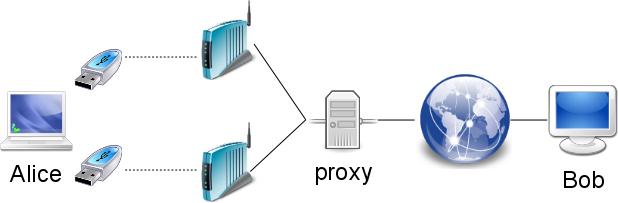
\includegraphics[width=\textwidth]{img/scenario}
\caption{\em Scenario}
\label{fig:scenario}
\end{figure}

La comunicazione VoIP tra i sistemi A e B si affida quindi a due tipi
di connessione: quella wireless, tra A e gli access point, e quella
via cavo tra gli access point e B.

\section{Vincoli qualitativi}
Come mostrato, il percorso dei dati da un sistema VoIP all'altro deve
attraversare segmenti camblati e altri senza fili; di questi gli
ultimi sono i più problematici, perché soffrono di tre gravi
inconvenienti: alta latenza, frequenti errori di trasmissione e
interruzione e ripristino della connessione nel cambiare access
point. Latenza ed errori frequenti possono degradare la qualità di una
comunicazione VoIP via wireless fino a renderla inintelleggibile,
mentre l'interruzione della connessione durante il passaggio da un
access point a un altro impedisce la mobilità del sistema obbligando
l'utente a restare nei pressi del ripetitore wireless in uso, pena la
disconnessione e l'interruzione della comunicazione.

Per garantire una buona qualità del servizio, il sistema RWMA deve
operare soddisfando vincoli di interattività, affidabilità e mobilità.

\subsection{Interattività}
L'interattività di una conversazione VoIP è influenzata dalla latenza
dei pacchetti che ne compongono il flusso di rete. La latenza di
trasmissione è definita come il tempo trascorso dall'istante del
campionamento della voce sul sistema di origine all'instante di
riproduzione audio della stessa voce sul sistema di destinazione. Le
raccomandazioni ITU--T \cite{bib:itu-t} indicano 150 ms come latenza
massima di una comunicazione VoIP soddisfacente; al di sopra di questa
soglia l'interattività della conversazione non è più accettabile.

\subsection{Affidabilità}
L'affidabilità di una conversazione VoIP dipende dalla capacità della
rete di portare a destinazione quanti più pacchetti possibili. Un
pacchetto è considerato perso quanto viene trasmesso dal sistema
origine e non viene ricevuto dal sistema destinazione. Per condurre
una conversazione comprensibile è necessario che la percentuale di
pacchetti persi resti al di sotto del 10\% \cite{bib:itu-t}. Poiché
per motivi di interattività le comunicazioni VoIP si svolgono su
protocollo UDP, la rete non offre nessun tipo di servizio di
trasmissione affidabile.

\subsection{Mobilità}
La mobilità dell'utente è fortemente limitata dallo scarso raggio
d'azione offerto dalle attuali apparecchiature WiFi. Le interfacce
WiFi sono in grado di interrompere l'associazione con l'access point
in uso per crearne una nuova con un secondo solo quando i suddetti
access point sono parte della stessa infrastruttura di rete. Questa
limitazione deriva direttamente dal funzionamento del protocollo IP:
cambiando rete di accesso l'interfaccia wireless riceve un nuovo
indirizzo IP e deve reinstaurare la connessione da zero. Ciò che si
vuole è invece un processo di disconnessione e riconnessione
trasparente all'applicazione, in modo che la chiamata VoIP non venga
interrotta, e rapido, in modo da non violare il requisito di
interattività precedentemente esposto.

\section{Il meccanismo RWMA}
Il meccanismo RWMA è costituito da più componenti, schematizzati in
figura \ref{fig:rwma}, che cooperano per risolvere i tre problemi di
interattività, affidabilità e mobilità. Questa sezione presenta
brevemente i componenti e illustra il loro ruolo nel progetto.
\begin{figure}[tb]
\centering
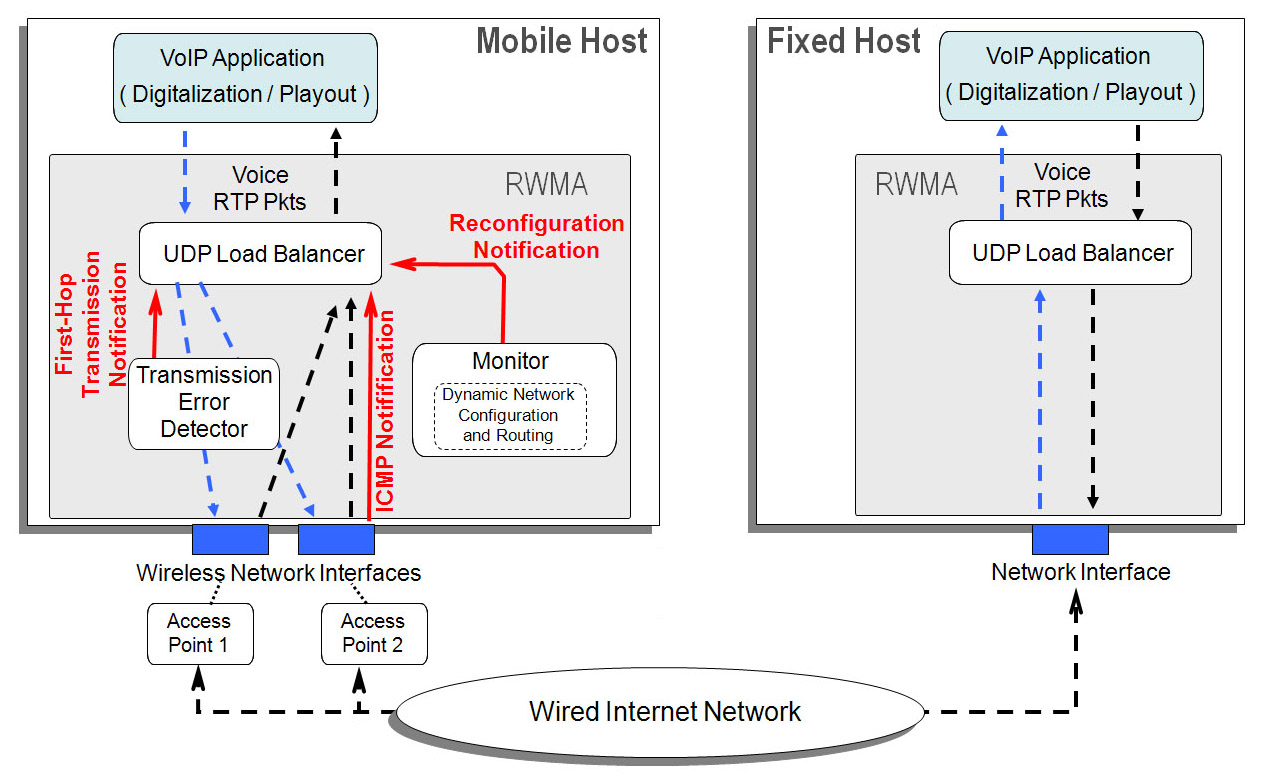
\includegraphics[width=\textwidth]{img/rwma}
\caption{\em Schema del meccanismo RWMA}
\label{fig:rwma}
\end{figure}

\subsection{Transmission Error Detection (TED)}
Questo componente software è integrato nel kernel del sistema
operativo del dispositivo mobile e ha il compito di tenere sotto
costante osservazione l'esito dell'invio dei pacchetti sulle
interfaccie wireless. Ogni volta che un'interfaccia WiFi invia un
\emph{frame} 802.11, questa deve attendere che l'access point risponda
con un frame di \emph{acknowledgment} che confermi l'avvenuta
ricezione. Nel caso in cui questo frame non venga ricevuto entro un
certo periodo di tempo, l'interfaccia ritenta la trasmissione fino a
un certo limite di volte, raggiunto il quale il frame viene
scartato. Se l'interfaccia riceve l'ACK, il firmware notifica il
kernel dell'avvenuta ricezione; al contrario, se il numero massimo di
tentativi viene raggiunto senza che l'interfaccia abbia ricevuto un
ACK, il firmware notifica il kernel del fallimento. Compito del TED è
rilevare queste notifiche positive e negative inviate dal firmware
dell'interfaccia e metterle a disposizione di applicazioni in
\emph{user space}.

\subsection{UDP Load Balancer (ULB)}
Questo componente software è un'applicazione in \emph{user space}
eseguita sul dispositivo mobile e ha il compito di rilevare le
notifiche di TED, e in base a queste decidere se rispedire i datagram
che non sono stati ricevuti dall'access point; inoltre deve valutare
di volta in volta quale sia l'interfaccia WiFi migliore da impiegare
per l'invio dei datagram.

\subsection{Interface Monitor (IM)}
Questo componente software lavora a stretto contatto con il gestore
delle interfacce wireless del sistema mobile e notifica ULB
dell'attivazione e della disattivazione di ogni interfaccia; dalle
notifiche di IM, ULB è quindi in grado di conoscere in ogni momento
quali interfacce wireless siano attive e associate a un'access point e
tra queste scegliere la migliore da usare per l'inoltro dei datagram.

\subsection{Proxy Server (PS)}
Questo componente software ha il compito di nascondere la mobilità del
sistema A, in modo che questo possa essere continuamente raggiungibile
dal sistema B. Il sistema B è in comunicazione con PS ed è
quest'ultimo a occuparsi di tenere traccia dei cambiamenti di
indirizzo IP che occorrono quando il sistema A cambia rete WiFi o
riattiva un'interfaccia di rete; come ULB, anche PS deve decidere a
quale interfaccia inoltrare i datagram ricevuti da B, ma a differenza
di ULB non si occupa di ritrasmettere eventuali pacchetti persi.

\chapter{Simulazione}
% Obiettivi a cui punto. Spiegazione soluzioni, algoritmi e scelte
% effettuate.
Tra i componenti del sistema RWMA descritti nel capitolo precedente,
UDP Load Balancer e Proxy Server ospitano il meccanismo su cui si basa
la qualità del servizio. Tutti gli altri meccanismi si occupano di
rilevare e trasmettere notifiche di errori o successi durante l'invio
di un datagram, quindi il comportamento è molto ben definito. ULB e PS
invece hanno il compito molto generico di dover scegliere
l'interfaccia \emph{migliore} per l'invio di ogni datagram. Gli
algoritmi di ULB e PS devono pertanto scegliere una definizione
operativa di ``migliore'' e applicarla alle interfacce WiFi in
uso.

In prima approssimazione un'interfaccia WiFi si può definire migliore
di un'altra quando offre maggiori probabilità di soddisfare i vincoli
di interattività e affidabilità descritti nel precedente capitolo; in
altre parole quando le stime di latenza e percentuale di pacchetti
persi per una data interfaccia sono le più basse tra le stime delle
altre interfacce attive.

Esistono vari modi per condurre queste stime, difficili da valutare
senza condurre test e misurazioni sul campo. La simulazione vuole
essere un banco di prova sperimentale virtuale, in cui condurre test
in maniera più comoda ed economica che nel mondo reale.

Scopo della simulazione è quindi confrontare diversi algoritmi di
stima della qualità delle interfacce WiFi per i componenti UDP Load
Balancer e Proxy Server.

Le sezioni successive mostreranno i problemi incontrati e le soluzioni
proposte.

\section{UDP Load Balancer}
Questa sezione illustra i problemi che devono essere affrontati dagli
algoritmi implementati dal componente ULB.

\subsection{Ritrasmissione in tempi brevi}
ULB deve attendere le notifiche del TED e ritrasmettere i datagram che
sono stati segnalati come persi, ma senza superare i 150 ms di
ritardo. Dopo tale periodo di tempo, un datagram voce viene
considerato \emph{stale} (scaduto) e quindi scartato. Inoltre la
ritrasmissione di un datagram causa l'attesa di tutti gli altri
datagram in coda; se ULB impiega troppi tentativi per ritrasmettere un
datagram, quelli successivi hanno meno tempo a disposizione per uscire
dal sistema prima di scadere. Il rischio è di far scadere una serie di
pacchetti solo per aver impiegato troppo tempo nella ritrasmissione di
uno. In particolare, ogni datagram contiene circa 40 ms di voce,
quindi ULB riceve i datagram da inoltrare a intervalli di circa 40 ms;
ogni datagram ha quindi 40 ms in cui può impegnare l'interfaccia
designata senza rubare tempo agli altri datagram in coda. Se ULB
dedica molto più di 40 ms all'invio di un datagram, rischia di
compromettere l'intera coda.

La soluzione proposta è di permettere una sola ritrasmissione per
datagram e di assegnare una valutazione negativa all'interfaccia che
ha ricevuto la notifica d'errore d'invio dal componente TED. In questo
modo la ritrasmissione di un pacchetto non blocca lo smaltimento degli
altri pacchetti in coda e la valutazione negativa all'interfaccia
problematica permette all'altra interfaccia designata per l'invio.

\subsection{Valutazione interfacce -- ULB}
ULB deve stimare la qualità di ogni interfaccia WiFi osservando le
notifiche ricevuto da TED.

TODO: algoritmo valutazione interfaccia, lo scrivo per ultimo a scanso
fix dell'ultimo momento.

\subsection{Rilevazione delle capacità del firmware}
I firmware delle schede di rete wireless sono in grado di notificare
sia l'avvenuta trasmissione di un datagram (ACK), sia la mancata
trasmissione (NACK). Normalmente le schede WiFi in commercio sono in
grado di notificare entrambi i casi, ma alcuni firmware sono in grado
di notificare solo ACK, oppure solo NACK. Mancando un meccanismo nel
kernel Linux per conoscere con certezza le capacità di ogni firmware,
ULB deve dedurrne il tipo dalle notifiche ricevute da TED. Conoscere a
priori il tipo di notifiche che possono giungere da un'interfaccia è
importante perché in caso di firmware che non possa segnalare i
fallimenti, ULB deve supplire a questa mancanza impostando un timeout
di ritrasmissione.

\subsubsection{Il problema del firmware silenzioso}
Il tipo di firmware si deduce dal tipo di notifiche ricevute dallo
stesso ed è quindi un meccanismo banale. Esistono però due casi in cui
il firmware può rimanere ``silenzioso'' e quindi impossibile da
rilevare: quando una connessione pessima, cioè che perde tutti i
pacchetti, viene gestita da un firmware ACK che notifica solo
successi, oppure quando una connessione ottima, ovvero che non perde
nessun pacchetto, viene gestita da un firmware NACK che notifica solo
fallimenti.

Non esiste un comportamento predefinito che soddisfi entrambe le
situazioni: la strategia del ritrasmettere ogni datagram che non
riceva notifiche entro un certo timeout funziona solo nella prima
situazione e risulta completamente inadeguato nella seconda.

\subsection{Valutazione interfacce -- PS}
Poiché il sistema mobile è dotato di più interfacce, PS si trova
nella necessità di scegliere a quale di queste debba inoltrare i dati
ricevuti dal sistema fisso.

La soluzione proposta consiste nel rispondere all'interfaccia che ha
spedito gli ultimi dati ricevuti; in altre parole inviare i dati
all'ultimo indirizzo IP da cui PS ha ricevuto traffico.

Può però accadere che il sistema mobile non invii alcun dato perché
l'utente si limita ad ascoltare; in questo caso il PS non ha
cognizione di quale sia l'interfaccia a cui inviare i dati.

TODO: soluzione PING, forse verrà già detta nella sezione ULB

\chapter{Simulatore}
Questo capitolo descrive brevemente l'implementazione del simulatore
progettato per la valutazione degli algoritmi ULB e PS.

Il simulatore è di tipo a eventi discreti ed è costituito da tre
strati.

Il primo strato è denominato \emph{de-sim} e costituisce un
\emph{framework} generico che definisce le classi di base da estendere
per modellare gli oggetti e i collegamenti, implementa la gestione di
eventi ed errori, l'instaurazione di collegamenti tra oggetti e
definisce primitive di input e output per lo scambio di oggetti tra
attori collegati.

Il secondo strato è denominato \emph{ulb-sim} e si basa su de-sim
estendendone le classi e specializzandone i metodi, per modellare una
versione semplificata del meccanismo RWMA.

Il terzo strato è denominato \emph{ulb-snr} e descrive lo scenario da
simulare instanziando le classi definite in ulb-sim e inizializzando
gli oggetti e gli eventi di partenza.

In altre parole, de-sim definisce come i meccanismi della simulazione,
ulb-sim gli oggetti partecipanti e infine ulb-snr dispone i
partecipanti nello scenario che si vuole raffigurare.

L'architettura a strati serve a mantenere indipendenza tra ciò che
definisce il ``cosa'' (ulb-sim) e ciò che definisce il ``come''
(ulb-snr): per esempio è possibile costruire nuovi scenari basati su
ulb-sim senza modificarne il codice.

Questra struttura è simile a quella del simulatore ns-2, in cui gli
oggetti della simulazione sono definiti da una gerarchia di classi in
C++, mentre gli scenari vengono definiti attraverso script Tcl
\cite{bib:ns-2}.

I tre strati sono scritti in Common Lisp \cite{bib:clhs}.

È importante notare che, a questo stadio di sviluppo, il simulatore
non punta al realismo fisico della simulazione. Per esempio, nelle
comunicazioni wireless non venendo presi in considerazione parametri
fisici come la qualità del segnale radio in relazione alla distanza
del client dall'access point. Tutti i dettagli di una connessione
wireless sono astratti dietro ai parametri di banda, latenza e
probabilità di errore; in particolare la rilevazione dell'ultimo
parametro sarà fondamentale per determinare la scelta dell'interfaccia
migliore. In quest'ottica, per simulare un calo di qualità del segnale
wireless dovuto all'aumentare della distanza tra client e access point
è sufficiente decidere quanto questo evento incida sulla probabilità
d'errore del collegamento e modificarla di conseguenza.

\chapter{Valutazioni}
TODO: Metriche con cui valuto il mio sistema. Deduzioni su misurazioni
effettuate. Perché ho misurato certe cose e non altre.

TODO: qui non ho la più pallida idea di cosa scrivere.

\chapter*{Conclusioni}
\rhead[\fancyplain{}{\bfseries
CONCLUSIONI}]{\fancyplain{}{\bfseries\thepage}}
\lhead[\fancyplain{}{\bfseries\thepage}]{\fancyplain{}{\bfseries
CONCLUSIONI}}
\addcontentsline{toc}{chapter}{Conclusioni}
TODO: che concludo?

\renewcommand{\chaptermark}[1]{\markright{\thechapter \ #1}{}}
\lhead[\fancyplain{}{\bfseries\thepage}]{\fancyplain{}{\bfseries\rightmark}}
\appendix
\chapter{Codice de-sim}
\rhead[\fancyplain{}{\bfseries Appendice \thechapter: Codice de-sim}]{\fancyplain{}{\bfseries\thepage}}
prova

\chapter{Codice ulb-sim}
\rhead[\fancyplain{}{\bfseries Appendice \thechapter: Codice ulb-sim}]{\fancyplain{}{\bfseries\thepage}}
prova

\end{comment}

\begin{thebibliography}{90}
\rhead[\fancyplain{}{\bfseries \leftmark}]{\fancyplain{}{\bfseries
\thepage}}
\addcontentsline{toc}{chapter}{Bibliografia}
\bibitem{bib:mipv6} RFC3775, ``Mobility Support in IPv6'',
  http://tools.ietf.org/html/rfc3775, giugno 2004
\bibitem{bib:misura-handoff-l2} A. Mishra, M. Shin, W. Arbaugh, An
  Empirical Analysis of the IEEE 802.11 MAC Layer Handoff Process, ACM
  SIGCOMM Computer Communication Review 33 (2), 2003.
\bibitem{bib:misura-handoff-dhcp} A. Dutta, F. Vakil, J. Chen,
  M. Tauil, S. Baba, N. Nakajima, H.  Schulzrinne, Application Layer
  Mobility Management Scheme for Wireless Internet, Proc. of IEEE 3G
  Wireless 2001, maggio 2001.
\bibitem{bib:mcoa} RFC5648, ``Multiple Care-of Addresses
  Registration'', http://tools.ietf.org/html/rfc5648, ottobre 2009
\bibitem{bib:hip} RFC5201 ``Host Identity Protocol'',
  http://tools.ietf.org/html/rfc5201, aprile 2008
\bibitem{bib:itu-t} ITU--T Recommendation G. 114, ``One--way
  Transmission'', maggio 2003
\bibitem{bib:banda-wlan} K. Medepalli, P. Gopalakrishnan, D. Famolari,
  and T. Kodama, Voice Capacity of IEEE 802.11b, 802.11a and 802.11g
  Wireless LANs, Proc. of Globecom 2004, pp.1549–1553, December 2004.
\bibitem{bib:abps} V. Ghini, G. Lodi, F. Panzieri, ``Always Best
  Packet Switching: the Mobile VoIP Case Study'', Achademy Plublisher,
  Journal of Communications, accepted for publication.
\bibitem{bib:abc} E. Gustafsson et al., ``Always Best Connected'',
  IEEE Comm. Mag., vol. 10, no. 1, Feb 2003, pp. 49--55.
\bibitem{bib:ns-2} http://nsnam.isi.edu/nsnam/, ottobre 2009
\bibitem{bib:clhs}
  http://www.lispworks.com/documentation/HyperSpec/Front/,
  ottobre 2009
\end{thebibliography}
\end{document}
